\chapter{Слежение для системы с астатизмом первого порядка (ПИ-регулятор)}
\label{ch:chap5}


Рассмотрим ПИ-регулятор следующего вида:
$$
H(s) = \frac{k_i}{s} + k_p
$$


\section{Движение с постоянной скоростью}
Будем пытаться угнаться за сигналом $g(t) = Vt = 2t$.
Выберем следующие пары коэффициентов $k$:

\begin{center}
  \begin{tabular}{ |c|c|c|c|} 
    \hline
    $k_i$  & 1   & 2  & 3 \\
    \hline
    $k_p$  & 4   & 5  & 6  \\
   \hline
   \end{tabular}     
\end{center}



Определим установившуюся ошибку, пользуясь теоремой о предельном значении:
$$
W_{g\to e} = \frac{1}{1+W(s)} = \frac{s^3 + 2.5s^2 + s}{s^3 + 2.5s^2 + (1+3k_p)s + 3k_i}
$$
$$
G(s) = \frac{V}{s^2}
$$
Образ ошибки слежения:
$$
E(s) = \frac{V(s^2 + 2.5s + 1)}{s(s^3 + 2.5s^2 + (1+3k_p)s + 3k_i)}
$$
В итоге:
$$
\begin{aligned}
  \lim_{t\to\infty} y(t) = \lim_{s\to 0}s\frac{V(s^2 + 2.5s + 1)}{s(s^3 + 2.5s^2 + (1+3k_p)s + 3k_i)} =  \\
  \lim_{s\to 0}\frac{V(s^2 + 2.5s + 1)}{s^3 + 2.5s^2 + (1+3k_p)s + 3k_i} = \dots \\
  \lim_{t\to\infty} y(t) = \frac{V}{3k_i} = \frac{2}{3k_i}
\end{aligned}
$$

Мы справились со слежением с точностью до установившейся ошибки, тоже неплохо.

Из таблицы выше мы получим следующие девять экспериментов:

\begin{figure}[ht]
  \centering
  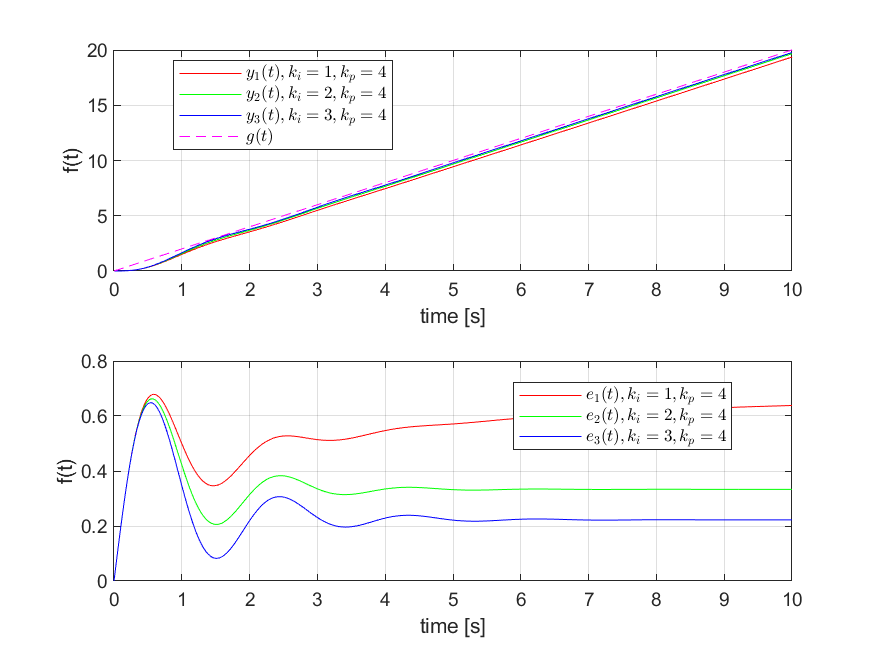
\includegraphics[width=0.8\textwidth]{output_task5_exp1.png}
\caption{Симуляция - движение с постоянной скоростью}
\end{figure}

\newpage
\begin{figure}[ht]
  \centering
  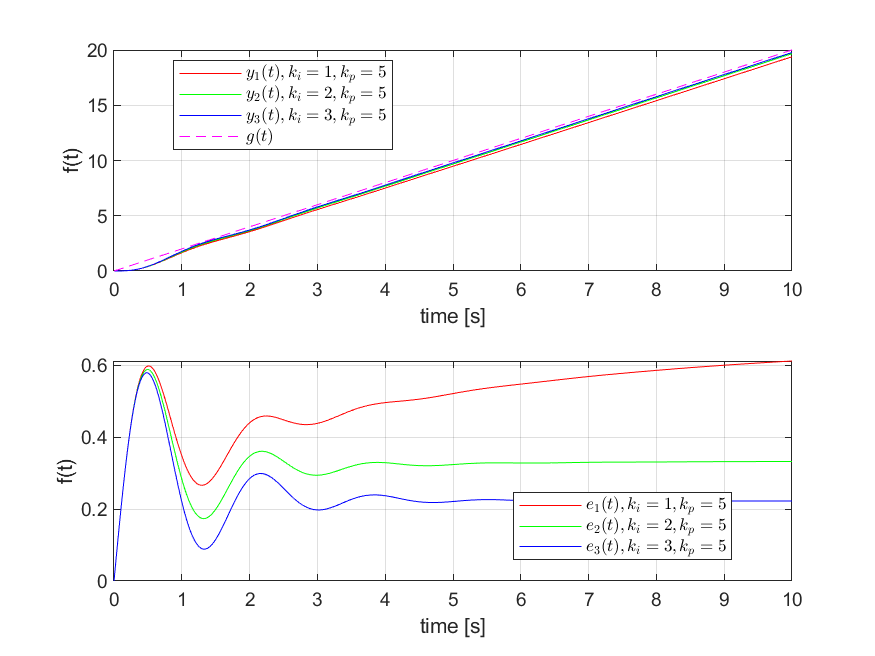
\includegraphics[width=0.8\textwidth]{output_task5_exp2.png}
\caption{Симуляция - движение с постоянной скоростью}
\end{figure}

\begin{figure}[ht]
  \centering
  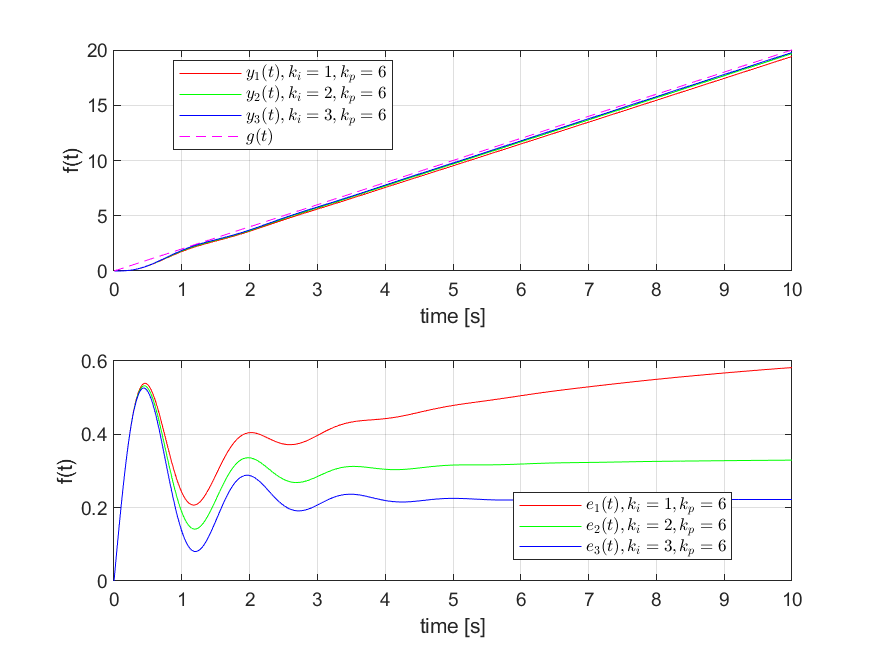
\includegraphics[width=0.8\textwidth]{output_task5_exp3.png}
\caption{Симуляция - движение с постоянной скоростью}
\end{figure}

\newpage
\begin{figure}[ht]
  \centering
  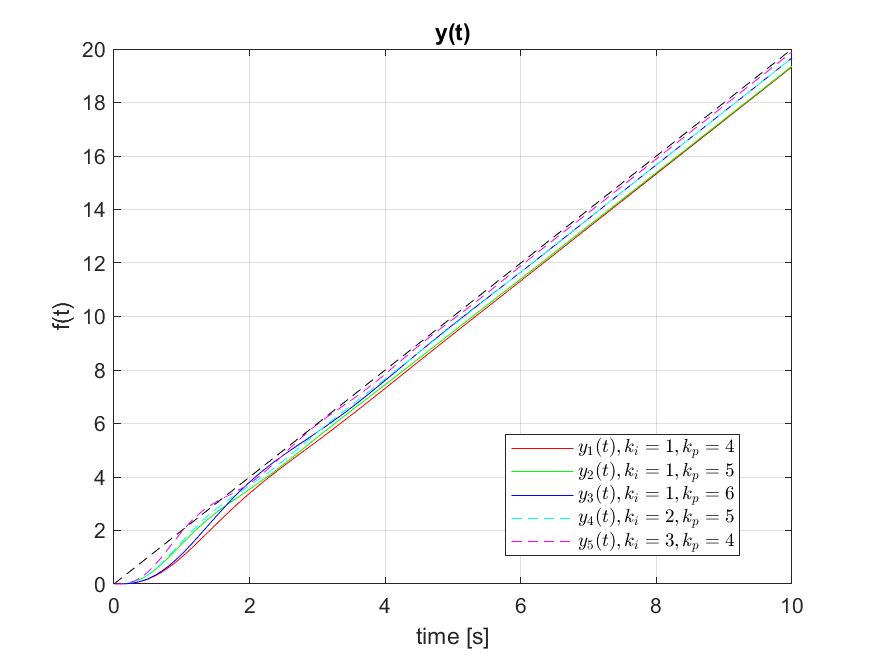
\includegraphics[width=0.8\textwidth]{output_task5_exp4.png}
\caption{Симуляция - движение с постоянной скоростью, сопоставление сигналов}
\end{figure}

\begin{figure}[ht]
  \centering
  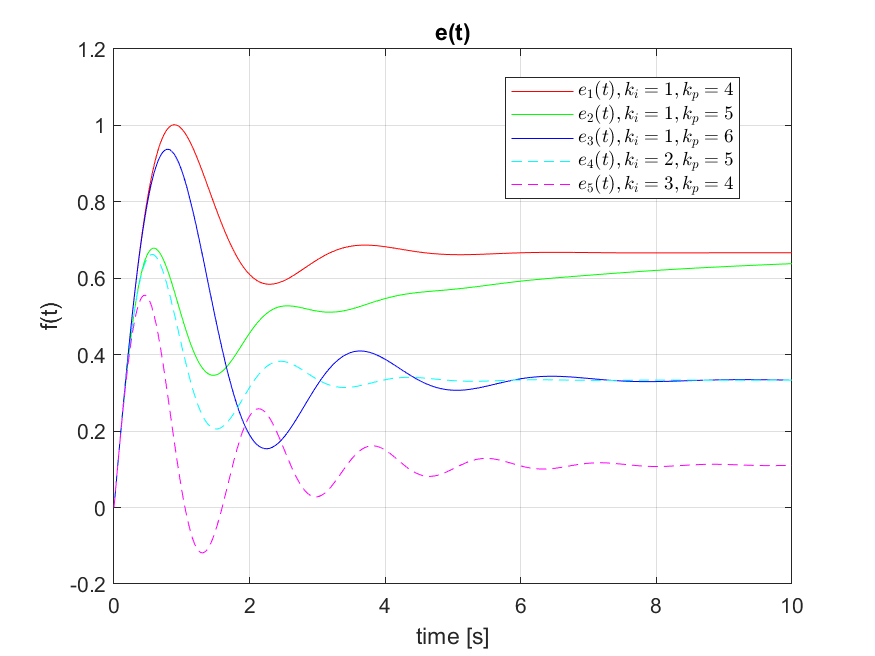
\includegraphics[width=0.8\textwidth]{output_task5_exp5.png}
\caption{Симуляция - движение с постоянной скоростью, сопоставление ошибок}
\end{figure}

\newpage
\textbf{Выводы:} При фиксированном $k_i$ уменьшение $k_p$ уменьшает время установления системы. Интегральный коэффициент, чем больше, тем больше амплитуда колебаний и меньше время установления. 
Для астатизма первого порядка выход системы y(t) совпадает с g(t) по наклону, но находится ниже на расстоянии установившейся ошибки. 
По графикам "слежения" можно подумать, что $y(t)$ и $g(t)$ совпадают, но это не так с точностью до установившейся ошибки, которая уменьшается обратно пропорционально $k_i$. 

\newpage
\section{Движение за гармоническим сигналом}

Будем пытаться угнаться за сигналом $g(t) = asin(\omega t) = 2sin(0.5t)$ в случае моего варианта.
Выберем следующие пары коэффициентов $k$:

\begin{center}
  \begin{tabular}{ |c|c|c|c|} 
    \hline
    $k_i$  & 1   & 2  & 3 \\
    \hline
    $k_p$  & 4   & 5  & 6  \\
   \hline
   \end{tabular}     
\end{center}



Определим установившуюся ошибку, пользуясь теоремой о предельном значении:
$$
W_{g\to e} = \frac{1}{1+W(s)} = \frac{s^3 + 2.5s^2 + s}{s^3 + 2.5s^2 + (1+3k_p)s + 3k_i}
$$
$$
G(s) = \frac{a\omega}{s^2 + \omega^2} = \frac{1}{s^2 + 0.25}
$$
Образ ошибки слежения:
$$
E(s) = \frac{s^3 + 2.5s^2 + s}{(s^2 + 0.25)(s^3 + 2.5s^2 + (1+3k_p)s + 3k_i)}
$$
По виду знаменателя (критерий Декарта) можно понять, что он будет содержать хотя бы один положительный корень, 
поэтому применить здесь предельную теорему не выйдет, мы не знаем что будет за ошибка, или $+\infty$ она.


\begin{figure}[ht]
  \centering
  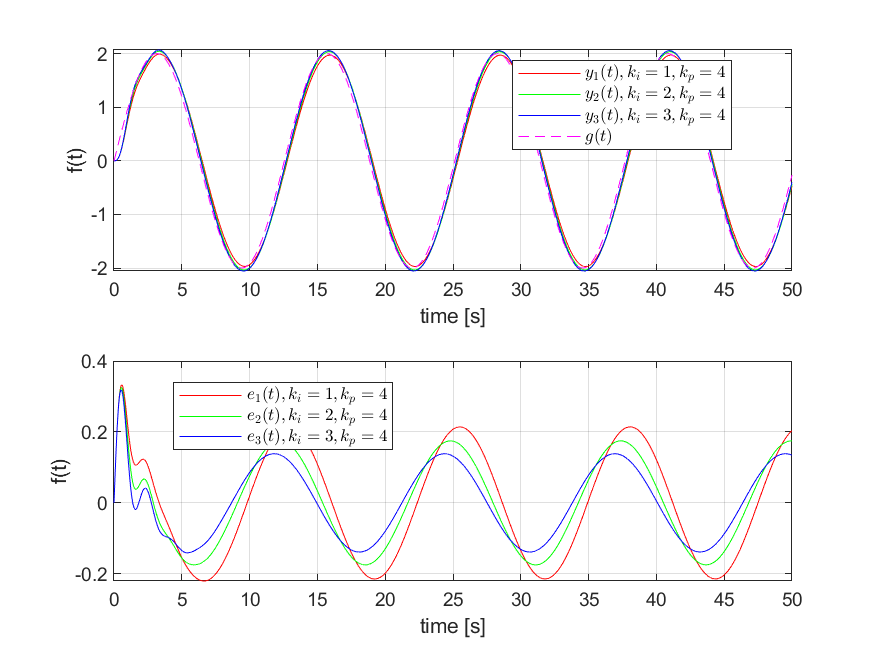
\includegraphics[width=0.8\textwidth]{output_task5_exp6.png}
\caption{Симуляция - гармоническое движение}
\end{figure}

\newpage
\begin{figure}[ht]
  \centering
  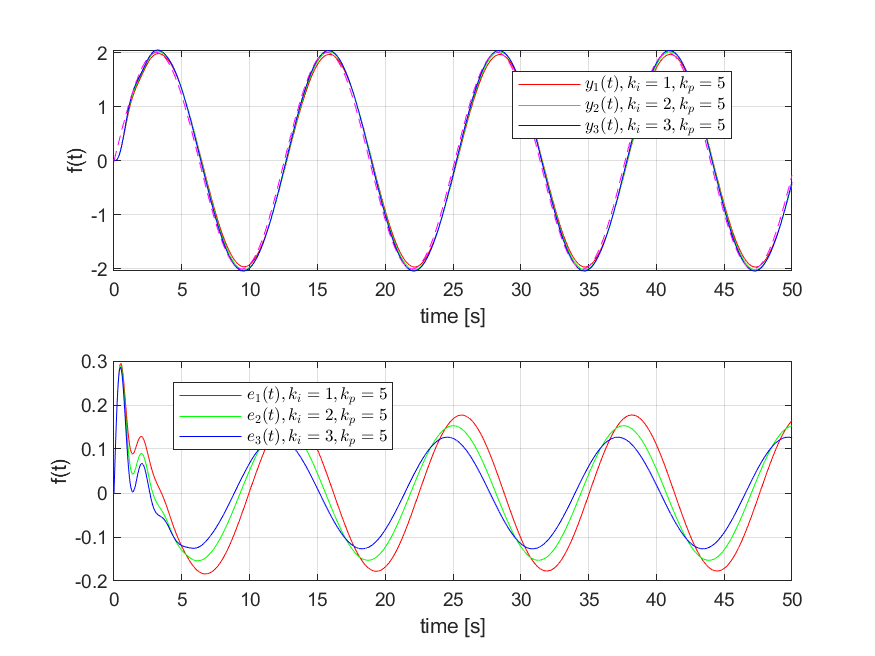
\includegraphics[width=0.8\textwidth]{output_task5_exp7.png}
\caption{Симуляция - гармоническое движение}
\end{figure}

\begin{figure}[ht]
  \centering
  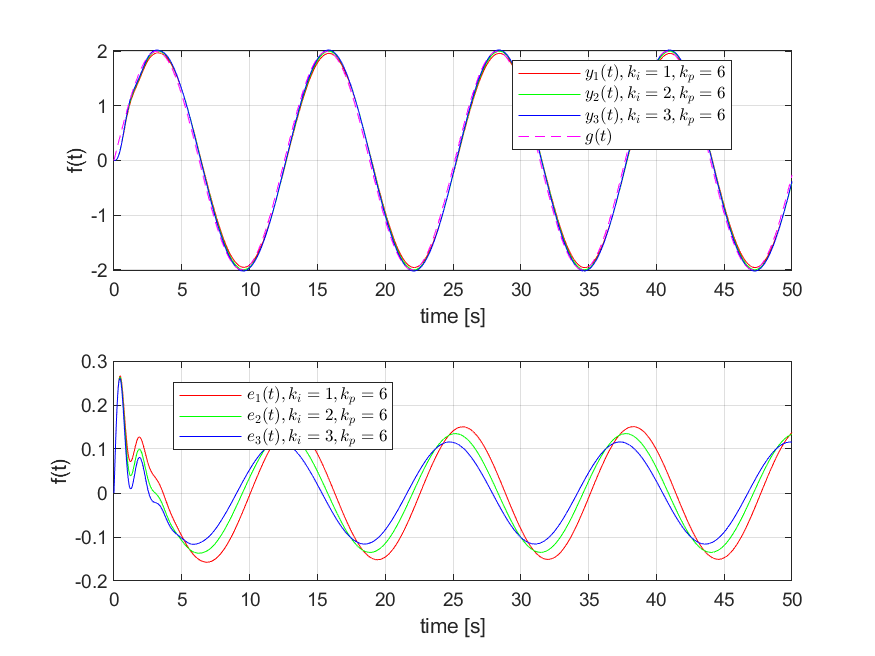
\includegraphics[width=0.8\textwidth]{output_task5_exp8.png}
\caption{Симуляция - гармоническое движение}
\end{figure}

\newpage
\begin{figure}[ht]
  \centering
  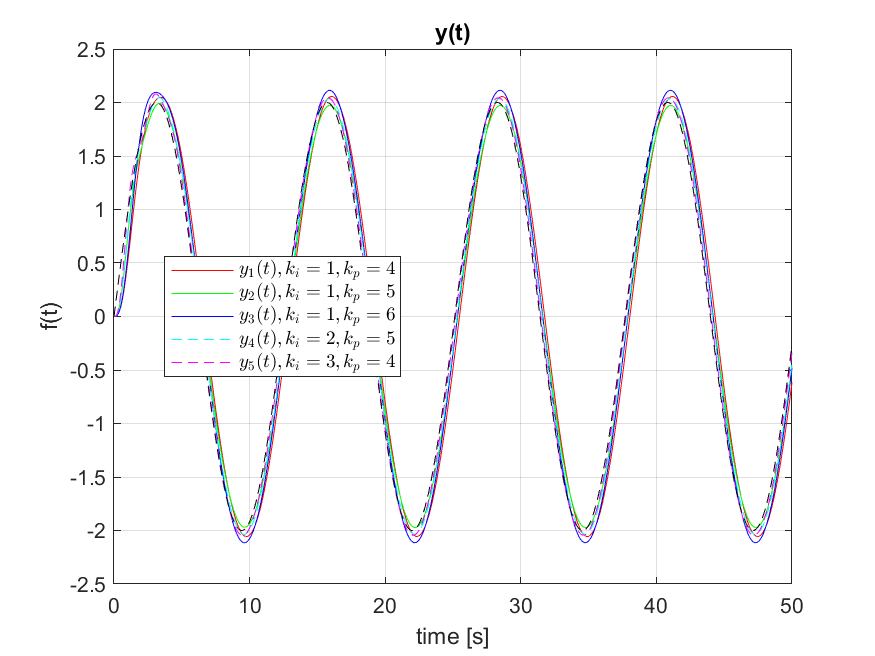
\includegraphics[width=0.8\textwidth]{output_task5_exp9.png}
\caption{Симуляция - гармоническое движение, сопоставление сигналов}
\end{figure}

\begin{figure}[ht]
  \centering
  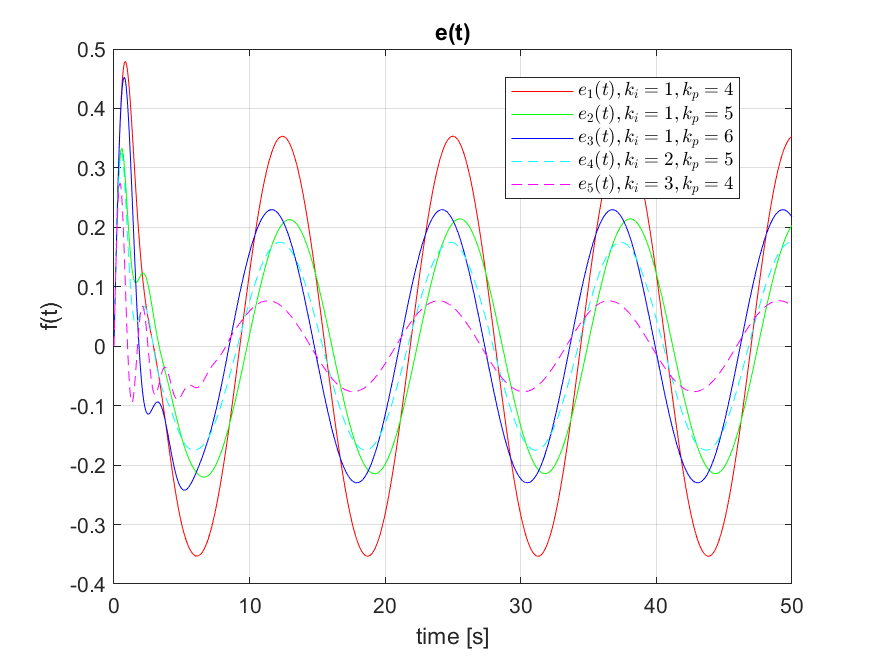
\includegraphics[width=0.8\textwidth]{output_task5_exp10.png}
\caption{Симуляция - гармоническое движение, сопоставление ошибок}
\end{figure}



\newpage
\textbf{Выводы:}  Увеличение $k_i$ уменьшает время установки системы и немного сглаживает колебания ошибки в начале(и наоборот). 
Чем больше $k_p$, тем выше пик у ошибки в начале и тем больше будет максимальная ошибка дальше(и наоборот).

\endinput